\chapter{Random Variables}
``A random variable can be compared with the holy roman empire: The Holy Roman Empire was not holy, it was not roman, and it was not an empire.'' - Some random guy in internet \\ 

From the first chapter, we have been using events and sample spaces to develop the idea of probability and calculating it. But, in practical world,  we have to link the events and sample spaces to \textbf{data}. This concept is called ``Random Variable'' or r.v shortly.
A Random Variable, in informal terms, places the $\Omega$ in real line so we can work with it more easily. There are still events, but in terms on Random Variables now.
\\From now on, we may write Random Variables as r.v or r.v. or r.vs or r.v or r.vs shortly for convenience.


%----------------------------------------------------------

\section{Introduction to Random Variables}

A Random Variable describes the data or the outcome $\omega$ as a real number. There is a reason this concept exists, since it opens new concepts for practical applications.
\newline
Let's begin with the formal definition of \textit{ Random Variable}.

\begin{definition}
    A \textbf{Random Variable X} is a function,
    $$ X \ : \ \Omega \rightarrow \mathbb{R}$$
    That assigns a real number $X(\omega)$ to each outcome $\omega$. \\
    In \textbf{layman terms}, a random variable is a way to assign a numerical code to each possible outcome. A r.v is \textbf{neither random, nor a variable.} It is just a function. 
\end{definition}

This concept is heavily used instead of sample spaces . From now on, sample space will be mentioned rarely. Think this way, when we work on functions in algebra or sometimes in calculus, we don't think about about the domain of the function, but the properties of function itself.
Here are some examples to understand the concept better.
\begin{example} Flip a coin. We know that $\Omega =\{H,T\}$. A r.v $X$ might assign $X(H) = 1$ and $X(T) = 0$. That is, heads is ``coded'' as 1 and tails is ``coded" as 0.
    
\end{example}
\begin{example}
    Flip a fair coin $n$ times. Let $X$ represent the number of heads we get. Then, $X$ is a random variable that takes values $\{0,1,2,...,n\}$.
\end{example}

\begin{example}
    Toss a fair six sided dice 2 times. Let $X$ be the sum of the two rolls we get. Then, $X$ is a random variable that takes values $\{2,3,4,...,12\}$.
\end{example}

\begin{example}
    A students wants to write a real number in intervals $[0,1]$. Let $X$ be the number student writes. Then, $X$ is also a random variable that takes any real numbers in that interval.
\end{example}

As you may guess, this extremely looks similar to events. Random Variables also have \textit{Independence, Conditional Random Variable, a probability function} and so on. Additionally , Random Variables can be either \textbf{Discrete} or \textbf{Continous}.
\par 
Discrete Random Variable's range is finite or countably infinite. The first two examples we gave are Discrete. Continuous Random Variables's range is uncountably infinite like the third example \newline

I want to emphasize  that Random Variables are neither random or a variable, they are functions. It is a bit hard to grasp the idea of this concept, so I highly recommend lurking in mathematical forums and try to understand it ( that is what I did). But in short, we use Random Variables instead of outcomes, since Random variables are \textbf{numbers}. Numbers are easier to work with, we can process the numbers, do algebraic operations to them, also they have a structure that outcomes do not.
Turn \textbf{ Example 2.1.1} to in sample space and events language, which is easier to work with? Bunch of $H,T$ or just a number?


%--------------------------------------------------------



\section{Distribution Functions c.d.f, p.m.f, p.d.f, p.p.f}
\subsection*{c.d.f and p.p.f}
We define  \textbf{Cumulative Distribution Function} as,

\begin{definition}
    The \textbf{Cumulative Distribution Function} or shortly \textbf{c.d.f} is a function $F_X \ : \ \mathbb{R} \rightarrow [0,1]$ such that
    \[ F_X(x) = P( X \le x) \]
    \textbf{Remark :} Every r.v (discrete and continuous) have c.d.f. For this reason, we can use c.d.f for unified treatment of r.v properties (that is, generalized concepts for all r.v). Moreover, c.d.f contains all the information about r.v, both continous and discrete ones. That is why c.d.f is very useful, even in practical world.
\end{definition}
\par
In informal terms, c.d.f is the probability that $X$ will take a value less than or equal to $x$. This property holds both for continuous and discrete r.v.


\begin{example}
    We toss a fair coin two times. Let $X$ represent the number of heads we get. Then c.d.f of $X$ is,
    \[F_X(x) = 
        \begin{cases} 
          0 \qquad &x < 0\\
          1/4 \qquad &0 \le x <1 \\
          3/4 \qquad &1 \leq x < 2 \\
          1 \qquad &x \ge 2
        \end{cases} 
\]
\end{example}

The variable $x$ can get $\textbf{any real numbers}$, such as $2, 4.14$ and $\pi$. It is just that in discrete case the probability equals to $0$ (Which in other words converts discrete to continous function?). It a bit tricky, they simply take the values from corresponding inequalities.
\\
Now, let's look at some properties of c.d.f,
\begin{theorem}
    Let $X$ have \textit{c.d.f} $F$ and $Y$  have \textit{c.d.f} $G$. If $F(x)=G(x)$ for all $x$, then,
    \[ P(X \in A) = P(Y \in A) \quad \text{for all $A$} \] 
\end{theorem}

\begin{theorem}
    the function $F \ : \mathbb{R} \rightarrow [0,1]$ is a c.d.f for some r.v if and only if $F$ satisfies three conditions:
    \begin{enumerate}
        \item $F$ is non-decreasing
        \item $F$ is normalized i.e \[ \lim_{x \rightarrow -\infty} F(x) = 0\ \ \land \ \lim_{x \rightarrow \infty} F(x) =1 \]
        \item $F$ is right continuous.
    \end{enumerate}
    \begin{proof}[Remarks]
        The first and second properties are simple and intuitive, therefore we will ignore them ( I know it is not the mathematical way, but whatever   ). \\
        
        Third property, however, is worth having discussion about. This property directly follows from the inequality $\le$. We could even define c.d.f with strict inequality $F= P(X<x)$, and it would still work. It is matter of convention.
    \end{proof}
\end{theorem}
\begin{definition}
    \textbf{Quantile Percent point function}, or shortly p.p.f, is defined as inverse of c.d.f i.e,
    \[Q(x) = F^{-1}(x)\]
\end{definition}
%------------------------------
\subsection*{c.d.f and p.d.f}
Similar to probabilities of Events, we can calculate probability of $X$ , depending on discrete or Continuous with functions called \textbf{ Probability Mass Function} and $\textbf{Probability Density Function}$, shortly $\textbf{p.m.f}$ and $\textbf{PDF}$ respectively,

\begin{definition}
    If $X$ is discrete, and it takes \textit{countably} values $ \{ x_1,x_2,..,
    x_n \}$ we define \textbf{Probability Mass Function} of X as follows:
    $$f_X(x)= P(X = x)$$
    Note that $P(X = x)$ is a function, not a number. We have to specify $x$ first to get a number.
    \textbf{Remark}: $ \{ X=x \} $ are disjoint events that form partition of $\Omega$.
\end{definition}

   With the properties of probability, we have $f_X \ge 0$ for all $x \in \mathbb{R}$ and $\sum_{i} f_X (x_i) =1 $. Let's revisit our Example 2.2.1

   \begin{example}
    We toss a fair coin two times. Let $X$ represent the number of heads we get. Then c.d.f of $X$ is,
    \[f_X(x) = 
        \begin{cases} 
          1/4 \qquad &x=0\\
          1/2 \qquad &x=1 \\
          1/4 \qquad &x=2\\
          0 \qquad &\text{otherwise}
        \end{cases} 
\]
\end{example}



Moreover, for any set of real numbers, $S$, we have
\[ P (X \in S) = \sum_{x \in S} f_X(x)\]
Since all $\{X = x \}$  are disjoint.\\
\par
We can apply similar rules to continuous r.vs,
\begin{definition}
    If $X$ is continuous, we can represent the probability distribution of $X$ with,
    \[ P(a < X < b) = \int_{a}^{b} f_X(x) dx \]
    Function  $f_X$ is called \textbf{Probability Density Function} or PDF as shortly.
\end{definition}
Nothing new here really, we just change the properties of p.m.f that we can use it on continuous r.vs. Now, let's look at some examples,\\
\par
You may noticed that c.d.f is similar to p.m.f and PDF. Indeed, the are related, c.d.f is just sum of these functions we defined over some interval $x$.
\begin{definition}
    c.d.f is related to p.m.f and PDF. For discrete r.vs,
    \[F_X(x) = P(X \le x) = \sum_{x_i \le x} f_X(x_i)\]
    And for continuous r.vs,
    \[F_X(x)= \int_{-\infty}^x f_X(x)dx \]
    And $f_X(x) = F_X^{'}(x)$ for for all differentiable points $x$.\\
  
    Note that this definition is heavily used instead of direct definitions above, since we can work with c.d.f only, and derive it to get needed functions.
\end{definition}
\par



%-------------------------------------------------------------------------------------


\section{Important Random Variables and their distribution}
\begin{definition}
    If $X$ has distribution $A$, we write
    \[ X \sim A\]
    Usually $A$ depends on some fixed numbers to define properly, we call them $\textbf{parameters}$. For example, the distribution \textbf{Bernoulli}$(p)$ has parameter $p$. We show parameters in c.d.f and p.m.f as,
    \[ f(x; parameters) \quad \text{and} \quad F(x; parameters) \]
    
\end{definition}
There are some specific examples of r.v. that are very useful in practical applications. We will show most important ones, and briefly discuss them. In later chapters, we will learn more about them. Note that we will write the notation with the name of the distribution.

\subsubsection{Degenerate distribution or Point mass distribution: $X \sim \delta_a$}
Consider tossing coin or dice where all the sides show the same value. The p.m.f is ,
\[f_X(x; \delta_a) = 1 \quad \text{for} \ x = a\]
You might guess why it is called degenerate sometimes. It is not random, but the distribution satisfies the definitions!
\subsubsection{Discrete Uniform distribution}
This distribution is the one of the most known ones. When there are finitely many values and each of them have the same probability, then $p = \frac{1}{n}$. Simple coin tossing, dice rolling are prime example of these. The p.m.f is,
\[f_X(x) = \frac{1}{n}\]
Where $x \in \{1,2,...,n \}$. Nothing new here.
for other cases, $f_X(x) = 0$. 
\subsubsection*{Bernoulli distribution: $X \sim \op{Bernoulli}(p)$ }
This distribution describes ``Yes or No'' type of experiments such as coin flipping. Therefore, $P(X = 1) = p$, $P(X = 0) = 1-p$. We can also calculate p.m.f,
\[f_X(x; p) = p^x(1-p)^{1-x} \quad \text{for} \ x \in \{0,1\}\]

\subsubsection*{Binomial distribution:  $ X \sim \op{Binomial}(n,p)$}
This distribution is generalized form of \textbf{Bernoulli distribution}. Similar to Bernoulli, this distribution describes ``Yes or no'' type of experiments, but for $n$ times of tries e.g tossing a coin $n$ times. Assuming tries are independent of each other, we can show p.m.f as,
\[f_X(x; n,p) = \binom{n}{x}p^x(1-p)^{n-x} \quad \text{for} \ x \in \{0,1,...,n\}\]
Notice that Binomial$(1,p)$ = Bernoulli$(p)$.
\subsubsection*{Geometric distribution: $X \sim \op{Geom}(p)$}
This distribution is also specified with Bernoulli. The geometric distribution describes the probability of the first occurrence of success requires after $x$ independent trials e.g getting the first head after $x$ tosses. The p.m.f is,
\[ f_{X}(x; p) = (1-p)^{x-1}p \quad \text{for} \ x \ge 1 \]
\subsubsection*{Poisson distribution: $X \sim \op{Poisson}(\lambda)$}
This distribution is mainly used for counts of events like photons hitting a detector in a time interval, number of car accidents, students achieving a low and high mark on exam, or number of pieces of chewing gum on a tile of a sidewalk. its p.m.f is,
\[f_X(x; \lambda) = e^{-\lambda} \frac{\lambda^{x}}{x!} \quad \text{for} \ x \ge 0 \]
Usually, $\lambda = rt$ where $r$ is average rate the events occur and $t$ is the time interval. The r.v $X$ represents the number of events.
\subsubsection*{Unfiorm distribution: $X \sim \op{Uniform}(a,b)$}
The p.d.f of $X$ is defined as,
\[f_X(x; a,b)= \frac{1}{b-a} \quad \text{for} \ x \in [a,b]\]
\subsubsection*{Normal (Gaussian) distribution: $X \sim N(\mu, \sigma^2)$ or $X \sim \mathcal{N}(\mu, \sigma^2)$}
This distribution is one of the most popular ones even for non-mathematician, layman people. The famous IQ graph, badly made ``memes'' are example of this. This distribution plays important role in statistics and probability. Moreover, we can observe this distribution in nature. p.d.f is defined as,
\[f_X(x; \mu, \sigma^2) = \frac{1}{\sigma \sqrt{2 \pi}}  e^{- \frac{(x- \mu)^2}{2\sigma^2}} \quad \text{for} \ x \in \R \]
We will learn about $\mu$ and $\sigma$ in later chapters. For now, just assume they are some random parameters. \\
We define  \textbf{standart Normal distribution} as $N(0,1)$, r.v as $Z$. This specific distribution is very important, so much that we show its p.d.f and c.d.f with new notation, namely $\phi(z)$ and $\Phi(z)$. There is no closed form expression for $\Phi(z)$. In modern days, the programming libaries calculate them. \\
It can be shown that we can show \textbf{any normal  probabilities} we want with $\Phi(z)$.
\subsubsection*{Exponential distribution: $X \sim \op{Exp}(\lambda)$}
This distribution is continous analogue of the geometric distribution. This distribution (and the ones after this) has complex properties so we will be brief with this.
We define its c.d.f as ,
\[f_X(x; \lambda) = \lambda e^{-x \lambda}\]
\subsubsection*{Gamma distribution: $X \sim \op{Gamma} (\alpha, \beta)$}
First, we start with a definition,
\begin{definition}
    For $\alpha > 0$, we define \textbf{Gamma function} as,
    \[\Gamma(\alpha) = \int_{0}^{\infty} t^{\alpha-1} e^{-t}dt\]
    It is generalized form of more simple and specific version, 
    \[ \Gamma(n) = (n-1)! \quad \op{for} \ n \in \mathbb{N} \]
\end{definition}
    We define p.d.f of $x$ as,
    \[f_X(x; \alpha, \beta) =  \frac{1}{\beta^{\alpha} \Gamma(\alpha)} x^{\alpha-1} e^{-x/ \beta} \quad x > 0\]
    Notice that $ \operatorname{Gamma}(1, \beta) =\operatorname{Exp}( \beta)$. That is, exponentional distribution is a specific case of gamma distribution.
    Gamma distribution itself is very useful and heavily used in this field. Moreover, we can derive more advanced ( which I have difficulties understanding) distributions from the gamma function. For now, we will end our discussion here.
%--------------------------

\section{Multivariate Distribution}
In practical word, we often work with multiple r.v in the same experiment. This can be a medical research with multiple tests, where tests are related with each other with the same sample space $\Omega$ and the same probability.\\
First, we define a special vector,
\begin{definition}
    Let $X_1,X_2,..,X_n$ be r.vs. We call $X = \{ X_1, X_2, ... ,X_n\}$ \textbf{a random vector}.
\end{definition}
\begin{definition}
    If r.vs $X_1,X_2,...,X_n$ are \textbf{independent} an have the same \textbf{marginal distribution} with c.d.f $F$, we define these r.vs as \textbf{independent and identically distributed}, shortly $\op{i.i.d}$, with notation,
    \[X_1,...,X_n \sim F\]
    similarly, we show the p.d.f the same way. i.i.d property is very important in statistical field.
\end{definition}
We can apply multivariate c.d.f as
\begin{definition}
    For $n$  r.v $\{ X_1,X_2,..,X_n \}$, the multivariate c.d.f $F_{X_1,X_2,...,X_n}$ is given by,
    \[F_{X_1,X_2,...,X_n}(x_1,x_2,...,x_n) = P(X_1 \le x_1,...,X_n \le x_n) \]
\end{definition}
There is nothing fancy here, actually. We simply redefine c.d.f in general sense for $n$ r.vs.
\par
Similarly, we can define multivariate p.m.f as,
\begin{definition} For random vector $X$,, the multivariate p.m.f  $f_{X_1,X_2,...,X_n}$ is given by,
    \[ f_{X_1,X_2,...,X_n}(x_1,x_2,...,x_n) = P(X_1=x_1 ,...,  \ X_n = x_n) \]
    This is generalized form of p.m.f

\end{definition}
Similarly, we define,
\begin{definition}
    We know that c.d.f and p.d.f are related by derivative. Then,
    For random vector $X$, the multivariate p.d.f $f_{X_1,..,x_N}$ is given by,
    \[f_{X_1,X_2,...,X_n}(x_1,x_2,...,x_n) = \frac{{\partial}^nF_{X_1,..,X_n}(x_1,...,x_n)}{\partial x_1\partial x_2...\partial x_n}\]
\end{definition}

The Properties and theorems are similar, but are generalized for $n$ r.vs.

\section{Marginal Distribution}
If more than one variable is defined in an experiment, it is important to distinguish between the multivariate probability of $(X_1,X_2,..,X_n)$ and individual probability distributions of $X_1,X_2,..,X_n$\\

Formally, \textbf{Marginal distribution is the probability of a single event (or r.v) occuring, independent of other events}. Therefore implementing marginal distributions are rather easy. In multivariate distributions, we redefine the needed variable as a ``constant'' and work with other variables only.
\begin{definition}
    If $X$ is a random vector with p.m.f $f_{X_1,X_2,..,X_n}$, then we define marginal distribution as,
    \[f_{X_1}= P(X_1 = x_1)= \sum_{x_1 \ constant} P(X_1=x_1,..,X_n=x_n)= \sum_{x_1\ constant} f_{X_1,X_2,..,X_n}(x_1,x_2,...,x_n)\]
\end{definition}
Similarly,
\begin{definition}
    We define marginal p.d.f as ,
    \[f_{X_i}(x_i) =  \int \int \int ... \int f(x_1,x_2,..,x_n)dx_1..dx_{i-1}dx_{i+1}...dx_n \]
\end{definition}
Similarly, c.d.f follows the same rule. $F_X(x)= F(x,a,b,c,...)$. \\
\textbf{Remark:} Marginality and conditionality are not the same thing. They look similiar, but their definitions are subtly different.
\par
%------------------------
\section{Independence}
Similar to events, r.vs also can be independent,
\begin{definition}
    Two r.vs $X$ and $Y$ are \textbf{independent} if, for every $A$ and $B$,
    \[P(X \in A, Y \in B)= P(X \in A)P(Y \in B)\]
    The definition persists for multivariate distributions.
\end{definition}
To check Independence, we need to check the above question for every subsets $A,B$. Additionally, we have the theorem,
\begin{theorem}
    Let $X$ and $Y$ have p.m.f $f_{X_y}$. THen $X$ and $Y$ are independent only and only if ,
    \[f_{X,Y}(x,y)=f_X(x)f_Y(y) \]
    The definiton persists for multivariate distributions.
\end{theorem}


%--------------------------
\section{Conditioning}
Similar to events, r.v $X$ can also have conditional distributions given that we have $Y=y$. We show the conditionality with,
\begin{definition}
    We can show conditional distribution of $X$ respect to $Y$ with,
    \[P(X=x| Y=y) = \frac{ P(X=x,Y=y)}{P(Y=y)} \]
\end{definition}
Moreover we can also define \textbf{conditional p.m.f} as,
\begin{definition}
    p.m.f of $X$ conditional respect to $Y$ can be written as 
    \[ f_{X|Y}(x|y)= \frac{f_{X,Y}(x,y)}{f_Y(y)}\]
\end{definition}
 

%---------------------
\section{Transformations of a Random Variable}
In some applications, we really are interested in distributions of some function of $X$. We call this concept \textbf{Transformation of X}.
\begin{definition}
    Let $X$ be r.v with PDF/p.m.f $f_X$ and c.d.f $F_X$. Let $Y=r(X)$ i.e $Y=X^2$ or $Y = \ln X$. We call $Y=r(X)$ \textbf{transformation of x}. \\
    \newline
    If $Y$ is discrete, p.m.f is given by,
    \[f_Y(y)= P(Y=y) =  P( r(X) = y) = P( \{x \ : \ r(x) = y\})= P( X \in r^{-1}(y)) \]
    \newline
    If $Y$ is continuous, we first calculate c.d.f and find derivative of it. 
    \begin{align*}
        F_Y(y) &= P( Y \le y) = P(r(X) < y) \\
               &= P(\{x \ : \ r(x) \le y \}) = P( A_y)    \\
               &= \int_{A_y} f_X(x)dx
    \end{align*}
    And the last step, $f_Y(y) = F^{'}(y)$.
\end{definition}
We can also generalize this concepts for Multivariate distributions, which we just increase dimensions we work with (too lazy, add this later).
t
\section{References}
\begin{enumerate}
    \item MIT
\end{enumerate}
\section{Exercises}
\begin{enumerate}
    \item Suppose $Z$ is a standard normal random variable. Use R to:
        \begin{enumerate}
            \item plot its p.d.f and c.d.f in the same plot
        \end{enumerate}
        \textbf{Solutions:}\\
        \begin{enumerate}
            \item R already has its own unique functions that would be extremely helpful for us \\
                \inputminted{R}{src/chapter2/standardnormalplot.R}
                \begin{center}
                    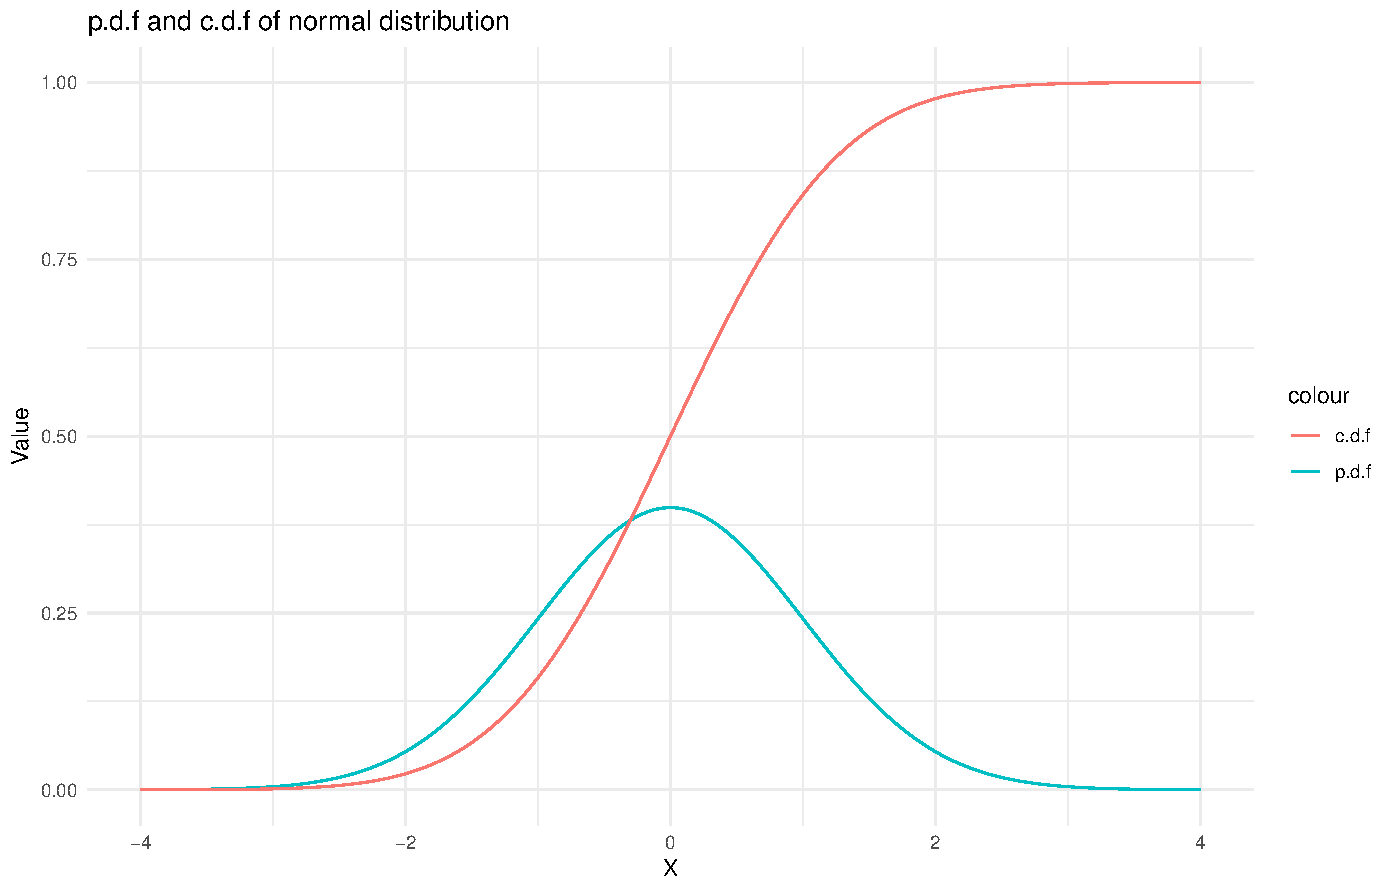
\includegraphics[width=1\textwidth]{src/chapter2/plot.pdf}
                \end{center}
        \end{enumerate}
\end{enumerate}
